% !TeX spellcheck = de_DE

\documentclass[12pt,a4paper,parskip=half]{scrreprt}

\usepackage[ngerman]{babel}
\usepackage[utf8]{inputenc}
\usepackage{acronym}
\usepackage{graphicx}
\usepackage[below]{placeins}
\usepackage{url}
\usepackage{hyperref}
\usepackage{tabularx}
\usepackage{booktabs}
\usepackage{textcomp}
\usepackage{caption}

% font coloring
\usepackage{xcolor}
% for tables
\usepackage{multirow}

\newcommand*{\captionsource}[2]{%
	\caption[{#1}]{%
		#1%
		\\\hspace{\linewidth}%
		\textbf{Quelle:} #2%
	}%
}

\title{Bericht Praxisphase I}
\author{Sebastian Wallat}
\date{\today}

\clubpenalty = 10000 % schliesst Schusterjungen aus
\widowpenalty = 10000 % schliesst Hurenkinder aus

\graphicspath{{./images/}}

\begin{document}

\begin{titlepage}
	
	\centering
	
%%	\ifcsempty{iodhbwm@institute@logo}{%
		
%%		
\includegraphics[height=1.5cm]{dhbw-logo}
		
	{%
		
		\begin{minipage}[c]{.25\textwidth}
			
			
\includegraphics[width=\textwidth, height = 2cm]{dhbw-logo}
			
		\end{minipage}
		\begin{minipage}[c]{0.46\textwidth}
			
			
\includegraphics[width=\textwidth]{empty}
			
		\end{minipage}
		\begin{minipage}[c]{.25\textwidth}
			
			\raggedleft
			
			
\includegraphics[width=\textwidth, height =2cm, keepaspectratio]{dlr-logo}
			
		\end{minipage}
		
	}
	
	
	
	\bigskip
	
	
	
	\Large\textsc{Große Studienarbeit}
	
	
	
	\normalsize
	
	des Studiengangs Informationstechnik\par
	
	der Dualen Hochschule Baden-Württemberg Mannheim
	
	
	
	\rule{\textwidth}{.5mm}\bigskip
	
	
	
	\textsc{\large Performance Analysis of serverless cloud functions}	
	
	
	\rule{\textwidth}{.5mm}
	
	
	
	\vfill
	
	
	
	\par
	
	{\bfseries\large Sebastian Wallat}\par
	
	3. Mai 2021
	
	
	
	\vfill
	
	
	
	\small{%
		
		\begin{tabularx}{\textwidth}{@{}lX@{}}
			
			\toprule
			
			
			Bearbeitungszeitraum: & 07.12.2020-05.05.2021\\
			
			Matrikelnummer, Kurs: & 1708267, TINF18-IT1\\
			
			Betreuer: & Dr. Frank Schulz \\
			
		\end{tabularx}
		
	}
	
	\cleardoublepage
	
\end{titlepage}


\newpage
\pagenumbering{Roman}

\chapter*{Eidesstattliche Erklärung}
%%\thispagestyle{empty}
\vspace{50pt}
Hiermit erkläre ich, dass ich die vorliegende Studienarbeit mit dem Titel ''Performance Analysis of serverless cloud functions'' selbständig verfasst habe, dass ich sie zuvor an keiner anderen Hochschule und in keinem anderen Studiengang als Prüfungsleistung eingereicht habe und dass ich
keine anderen als die angegebenen Quellen und Hilfsmittel benutzt habe. Alle
Stellen der Arbeit, die wörtlich oder sinngemäß aus Veröffentlichungen oder aus
anderweitigen fremden Äußerungen entnommen wurden, sind als solche kenntlich
gemacht. 

\vfill
\noindent\rule{5cm}{.4pt}\hfill\rule{5cm}{.4pt}\par
\noindent Datum, Ort \hfill Unterschrift 

\newpage
\thispagestyle{empty}
\chapter*{Zusammenfassung}

 Performance Analysis of serverless cloud functions
\\
Serverlose Architekturen gewinnen im Bereich des Cloud-Computing vermehrt an Bedeutung. Ein Vertreter hierfür sind serverlose Cloudfunktionen die mittlerweile von allen großen Cloud Service Providern (CSP) angeboten werden. Ziel dieser Arbeit soll es sein serverlose Cloudfunktionen auf ihre Performanz zu untersuchen.
\\
Dafür soll zuerst geklärt werden worum es sich bei serverlosen Funktionen handelt, sowie ihre Vor-und Nachteile kurz erläutert werden. Die Performanz-Analyse soll am Beispiel von AWS Lambda erfolgen.
\\
Zur Analyse sollen vier Test-Funktionen implementiert werden und auf verschiedene Eigenschaften, wie z.B. Latenz untersucht werden. Besonders die Coldstart-Problematik von serverlosen Systemen soll hierbei näher erläutert werden.
\\
Zum testen der Funktionen wird eine selbst einwickelte NodeJS Anwendung verwendet, welche die Funktionen ansteuert und die Ergebnisse Protokolliert. Zur Auswertung der so gesammelten Daten wird eine Jupyter-Notebook entwickelt, welches die gängigen Data-Science Bibliotheken wie Pandas und Matplotlib verwendet.


\bigskip


\tableofcontents
\addtocontents{toc}{}

\listoffigures
\addcontentsline{toc}{chapter}{Abbildungsverzeichnis} 
%%\thispagestyle{empty}

\newpage
\chapter*{Abkürzungsverzeichnis}
\addcontentsline{toc}{chapter}{Abkürzungsverzeichnis}
%%\thispagestyle{empty}
\begin{acronym}[HTTP]
	\acro{SaaS}{\textbf{S}oftware-\textbf{a}s-\textbf{a}-\textbf{S}ervice}
	\acro{CAD}{\textbf{C}omputer-\textbf{A}ided \textbf{D}esign}
	\acro{CSP}{\textbf{C}loud \textbf{S}ervice \textbf{P}rovider}
	\acro{AWS}{\textbf{A}mazon \textbf{W}eb \textbf{S}ervices}
	\acro{SLA}{\textbf{S}ervice \textbf{L}evel \textbf{A}greements}
	\acro{CSV}{\textbf{C}omma-\textbf{s}eparated \textbf{v}alues}
\end{acronym}

\pagenumbering{arabic}

\chapter{Einführung}
Durch die stetig voranschreitende Digitalisierung von Unternehmen gewinnen im Besonderen Cloud-Basierte Softwarelösungen an Bedeutung. Hierzu zählen unter anderem Software-as-a-Service (SaaS) Angebote wie Office356 von Microsoft (Textverarbeitung) oder Fusion360 von Autodesk (CAD-Programm). Des weiteren sind viele der heutigen Web-Anwendungen in der Cloud gehostet.  Alle diese Anwendungen haben gemein, dass die wesentliche Datenverarbeitung nicht auf dem Gerät des Nutzers erfolgt, sondern auf den Servern des Cloud Service Provider (CSP). Hierfür bieten die meisten CSP Baukastensysteme an um schnell komplexe Backend-Strukturen innerhalb ihrer Umgebung implementieren zu können. Einige Bespiele hierfür sind Datenbanksysteme, API-Gateways, Serverlose-Funktionen, (Container)-Hosting und weitere.
\\
Das Ziel dieser Arbeit ist es sich mit einem dieser Systeme näher zu beschäftigen, den Serverlosen Cloudfunktionen. Diese bieten die meisten CSP in ihrer Infrastruktur an, z.B AWS-Lambda (Amazon Web Services) und Google Cloud Run.
\\
Cloudfunktionen sind eine kostengünstige Lösung um bestimmte Backend Funktionalitäten zur Verfügung zu stellen. Sie sind zustandslose (stateless) Programmstücke, die über eine definierte Aktion aktiviert werden, z.B einen API Aufruf. Zur Ausführung erstellt der CSP einen neue Instanz der Funktion (falls nicht schon vorhanden) und führt diese aus. Die Besonderheit hierbei ist die zustandslösigkeit, also die Eigenschaft der Funktion keine persistenten Daten zu speichern. Alle für die Ausführung benötigten Daten, müssen vom Aufrufer mitgegeben werden, oder aus einer persistenten Datenquelle (z.b Datenbank) geladen werden. Da die Funktion aus diesem Grund nicht auf einem normalen Webserver läuft, sondern nur führ einen Aufruf existiert, werden sie auch als serverlos bezeichnet. \cite{Lambda-overview} 
\\
Der größte Vorteil von Cloudfunktionen gegenüber einem herkömmlichen Webserver, liegt darin, dass nur pro Aufruf kosten einstehen. Da ein normaler Webserver ja durchgängig Ressourcen des CSP belegt, fallen für ihn auch kosten an, wenn er nicht benutzt wird.
\\
Aus diesem Verhalten ergibt sich direkt auch ein wesentlicher Nachteil, der allerdings die meisten Cloud-Services betrifft, dieser liegt in der Varianz der Kosten. Erfreut sich ein Service unerwarteter Beliebtheit, so können unerwartet hohe Kosten durch den vermehrten Aufruf der Funktion entstehen.
\\
Dies wird besonders durch die gute horizontale Skalierbarkeit der Cloudfunktionen verstärkt. Würde ein traditioneller Webserver durch zu viele Anfragen überlastet, kann man von einer Funktion beliebig viele Instanzen erzeugen, welche die Anfragen parallel verarbeiten können.
\\
\\
Im weiteren Verlauf der Arbeit kann aus mehreren Gründen nur auf einen CSP eingegangen werden, hierfür wurde AWS ausgewählt. AWS stellt Cloudfunktionen unter seinem AWS-Lambda Service bereit. Daher sind die folgenden Ausführungen nur in der AWS Umgebung gültig und die präsentierten Resultate gelten nur für AWS-Lambda Funktionen.

\chapter{Technischer Hintergrund (AWS Lambda)}
AWS beschreibt Lambda folgendermaßen: ''AWS Lambda ist ein serverloser Datenverarbeitungsservice, der Ihren Code beim Eintreten bestimmter Ereignisse ausführt und für Sie automatisch die zugrunde liegenden Datenverarbeitungsressourcen verwaltet'' \cite{Lambda-overview}
\\
Dies lässt sich an einem kleinen Beispiel verdeutlichen:
\FloatBarrier
\begin{figure}[h!]
	\centering
	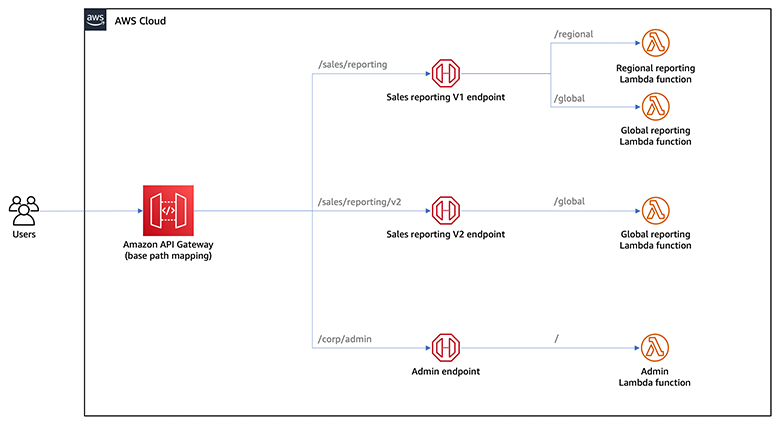
\includegraphics[width=14cm, height=8cm]{LambdaExample}
	\captionsource{Beispiel für den Einsatz von Lambda Funktionen mit einem API-Gateway als Auslöser}
		{https://aws.amazon.com/de/blogs/compute/icymi-serverless-q1-2021/}
	\label{AWS_Example}
\end{figure}

Grafik \ref{AWS_Example} zeigt die Verwendung von Lambda Funktionen in Kombination mit einem AWS API Gateway. Der Gateway besitzt mehrere vordefinierte Endpunkte, die jeweils mit einer Lambda-Funktion verknüpft sind. Schickt ein Nutzer eine HTTP Anfrage mit einem bestimmten Pfad (z.B ''/corp/admin'') an den die URL des API Gateway, so extrahiert dieser den konkreten Pfad der Anfrage und startet die verknüpfte Lambda-Funktion (in diesem Fall die ''Admin'' Funktion) mit den mitgelieferten Parametern.

\chapter{Performance Tests}

Ziel soll es sein AWS Lambda Funktionen auf ihre Performanz zu untersuchen. Als Kriterien hierfür bieten sich Latenz und Verfügbarkeit an.
\\
In den Service Level Agreements (SLA) von AWS Lambda garantiert AWS eine Verfügbarkeit von mindestens 99.95\% pro Monat. Sollte dies nicht erfüllt werden, so bekommt der Kunde eine Gutschrift für zukünftige Lambda Kosten, in Form sogenannter ''Service Credits''. Ab einer Verfügbarkeit von unter 95\% werden die gesamten Kosten als Service Credits gutgeschrieben.
\cite{Lambda-SLA}
\\
Weitere Informationen hierzu findet man in der offiziellen SLA von AWS Lambda (\url{https://aws.amazon.com/de/lambda/sla/})
\\
Da die Angaben der SLA dafür sprechen dass AWS von einer hohen Verfügbarkeit ausgeht und dies bei einem weltweit führenden CSP durchaus erwartet werden kann, soll die Verfügbarkeit nicht Fokus der weiteren Untersuchungen sein.
\\
Da die Lambda SLA keine Angaben zur Latenz machen, soll diese näher untersucht werden. Besonders die Problematik des sogenannten ''Cold start'' (zu deutsch Kaltstart) soll untersucht werden.

\section{Cold start (Kaltstart) von serverlosen Architekturen}
Aufgrund der serverlosen Architektur von AWS Lambda liegt die Vermutung nah, dass er Kaltstart wesentlichen Anteil an der Latenz einer Lambda Funktion haben könnte. Daher soll zuerst geklärt werden worin genau die Kaltstart-Problematik besteht.
\\
Da Lambda Funktionen keinen permanenten Server Prozess besitzen, sondern Instanz basiert sind, existieren zu einer bestimmten Zeit t eine bestimmte Anzahl von Instanzen n der Funktion. Wie groß n zu einem konkreten Zeitpunkt ist, wird von Skalierungsalgorithmen bestimmt und hängt in erster Linie von der Anzahl der Aufrufe in einem bestimmten Zeitfenster $\Delta$t ab. (vgl. Autoscaling von AWS Lambda \cite{Lambda-overview}).
\\
Um Ressourcen zu sparen wird die Anzahl der Funktions-Instanzen auf null reduziert, falls in einem festgelegten Intervall keine Aufrufe der Funktion stattfinden.
\\
Trifft nun ein neuer Aufruf für die Funktion ein, so muss der CSP zuerst eine neue Instanz erstellen, welche dann die Anfrage bearbeiten kann. Dies wird als Kaltstart bezeichnet (Skalierung von $n=0$ auf $n\geq1$)
\\
Die Gesamtzeit des (oder der) ersten Funktionsaufrufe(s) erhöht sich somit um die Zeit, die zur Instanziierung der Funktion benötigt wird. Je nach verwendeter Programmiersprache kann es zusätzlich passieren dass das Programm deutlich langsamer Ausgeführt wird als nach einiger Laufzeit (z.B JIT Laufzeitoptimierung von Java \cite{Java-JIT}). In diesem Fall vergrößert sich die Laufzeit nach Kaltstart zusätzlich.

\section{Testaufbau}
Um verschiedene Performance-Aspekte von AWS Lambda Funktionen zu untersuchen wurde der im folgenden näher beschriebene Testaufbau verwendet.

\subsection{AWS}

Der Testaufbau besteht aus 4 in AWS implementierten Lambda-Funktionen. Diese sind über einen API Gateway erreichbar.

\FloatBarrier
\begin{figure}[h!]
	\centering
	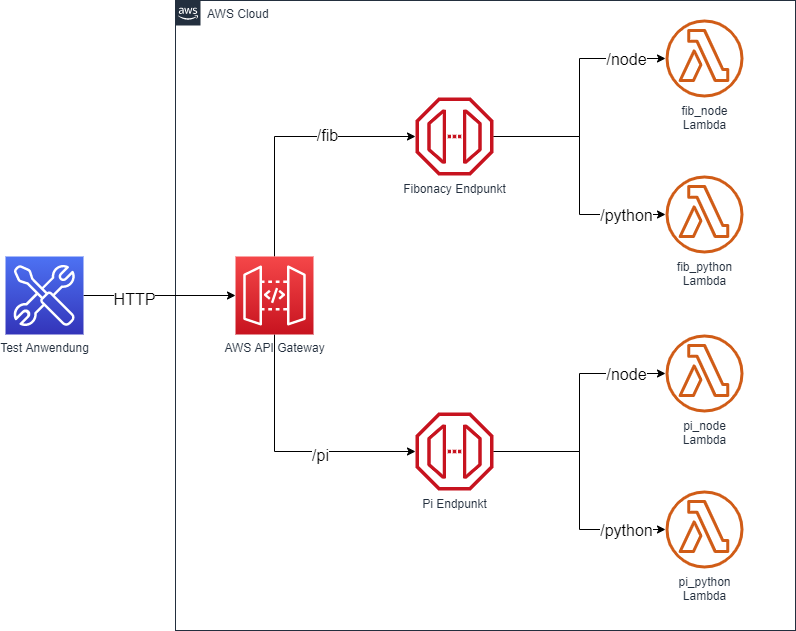
\includegraphics[width=14cm, height=10cm]{LambdaLayout}
	\captionsource{Überblick über die in AWS implementierten Funktionen}
	{Eigene Darstellung mit DrawIO}
	\label{Lambda_Aufbau}
\end{figure}

Darstellung \ref{Lambda_Aufbau} zeigt eine Überblickskizze über die in der Cloud implementierten Funktionalitäten. Insgesamt wurden vier Lambda-Funktionen implementiert, hierbei wurden zwei verschiedene Programmiersprachen und zwei Arten von Workloads berücksichtigt. Als verwendete Sprachen werden Python und Java Script (NodeJS-Framework) verwendet. Bei den implementierten Workloads handelt es sich einmal um die iterative Berechnung von $\pi$ auf eine festgelegte Anzahl stellen, sowie um die rekursive Berechnung einer Zahl der Fibonacci folge. Der Sourcecode kann unter folgendem Link eingesehen werden: \url{https://github.com/SebastianWallat/StudienarbeitAWS}
\\
Des weiteren dokumentiert jede Lambda Funktion ihre Laufzeit und sendet diese, sowie das Ergebnis der Berechnung an den Aufrufer zurück.


\subsection{Test-Anwendung}

Um die zuvor implementierten Funktionen zu testen wurde eine einfache NodeJS Anwendung entwickelt. Diese aktiviert die Lambda-Funktionen über ihre korrespondierenden API-Pfade und speichert die Ergebnisse als CSV. Hierbei misst die Applikation die Ausführungszeit der gesamten Http Get Anfrage (Roundtrip). Des weiteren wird die in der API Antwort enthaltene serverseitige Laufzeit, sowie der Http Statuscode gespeichert.
\\
Über eine CSV Datei (Timings.csv) kann eine Sequenz für das Durchführen der Abfragen angegeben werden, in dieser wird die Anzahl an derselben, sowie die Wartezeit zwischen den Anfragen festgelegt.
\\
Die nachfolgende Tabelle \ref{table:1} zeigt eine mögliche Request-Sequenz:
\begin{table}[h!]
	\centering
	\begin{tabular}{||c c||} 
		\hline
		Wartezeit (in ms) & Anzahl Aufrufe \\ [0.5ex] 
		\hline\hline
		1000 & 5 \\
		5000 & 10 \\[1ex] 
		\hline
	\end{tabular}
	\caption{Beispiel einer Abfragesequenz}
	\label{table:1}
\end{table}

Diese Tabelle kann folgendermaßen interpretiert werden:\\
Führe zuerst 5 Aufrufe mit jeweils 1 Sekunde Pause aus, danach führe 10 Aufrufe mit jeweils 5 Sekunden Pause aus.

\newpage
\section{Auswertung}

Zur Auswertung der gesammelten Daten wird ein Jupyter-Notebook (Python) verwendet, dieses visualisiert die Latenzzeiten unter Verwendung der üblichen Data-Science Frameworks (unter anderem Pandas, Matplotlib).
\\
Um eine relativ gute Datenbasis zu erhalten wurden alle versuche mindestens drei Mal durchgeführt und ihre Ergebnisse gemittelt.

\subsection{Client-Daten}

\FloatBarrier
\begin{figure}[h!]
	\centering
	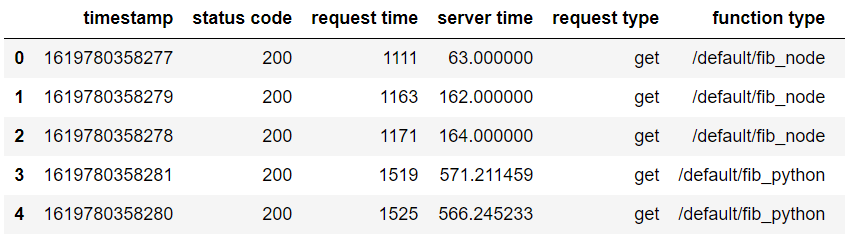
\includegraphics[width=13cm, height=4cm]{LocalDataExample}
	\captionsource{Ausschnitt aus den von der lokalen Test Anwendung gesammelten Daten}
	{Eigene Darstellung (Pandas)}
	\label{LocalDFHead}
\end{figure}
\FloatBarrier

Grafik \ref{LocalDFHead} zeigt einen Ausschnitt der gesammelten Daten. Diese werden innerhalb des Jupyter-Notebook zuerst für die Darstellung vorbereitet. Hierzu zählt unter anderem die Umwandlung des Zeitstempels in die vergangene Zeit seit Start der Anwendung. Dafür wird für jeden Zeitstempel die Differenz zwischen ihm und dem allerersten berechnet und das Zeitintervall in Millisekunden angegeben. Danach können die Daten in einigen Grafiken dargestellt werden.
\\

\FloatBarrier
\begin{figure}[h!]
	\centering
	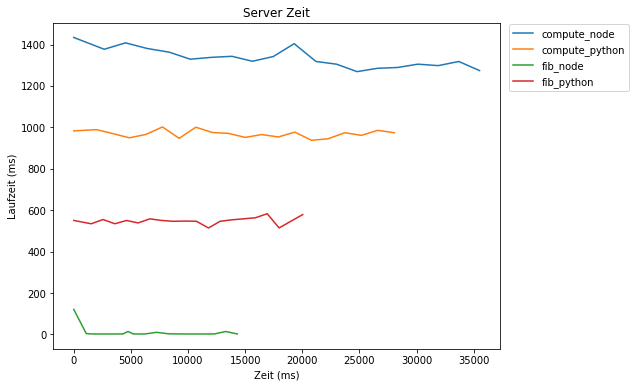
\includegraphics[scale=0.7]{aw_c_server_full}
	\captionsource{Serverseitige Laufzeiten der Lambda Funktionen}
	{Eigene Darstellung (Matplotlib)}
	\label{aw_c_server_full}
\end{figure}
\FloatBarrier

\FloatBarrier
\begin{figure}[h!]
	\centering
	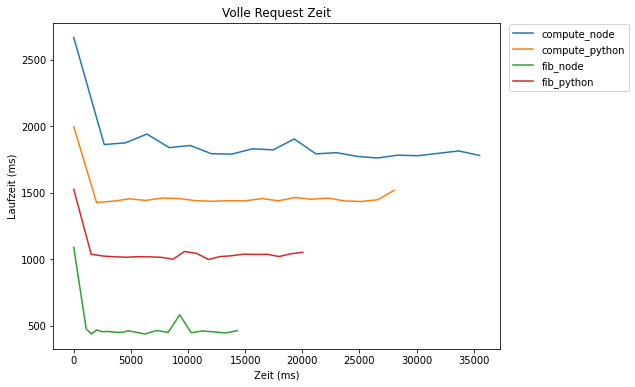
\includegraphics[scale=0.7]{aw_c_client_full}
	\captionsource{Laufzeiten des gesamten Funktionsaufrufs (Roundtrip)}
	{Eigene Darstellung (Matplotlib)}
	\label{aw_c_client_full}
\end{figure}
\FloatBarrier

Die Abbildung \ref{aw_c_server_full} zeigt die serverseitigen Laufzeiten aller vier Lambdafunktionen. Zu erkennen ist eine relativ konstante Ausführungszeit für jede Funktion, außer der NodeJS Fibonacci Implementierung, welche eine stark erhöhte bei ihrer ersten Ausführung aufweist.
\\

Abbildung \ref{aw_c_client_full} zeigt die Clientseitige Latenz der gesamten HTTP Abfrage (Roundtrip). Hier ist eine deutliche Erhöhung der Benötigten Zeit für die erste Antwort erkennbar. Dies lässt sie mithilfe des zuvor erläuterten Kaltstart-Problems erklären. Zur Verdeutlichung zeigen die nächsten zwei Grafiken nur die Anfragen die in den ersten 5 Sekunden des Tests erfolgt sind.

\FloatBarrier
\begin{figure}[h!]
	\centering
	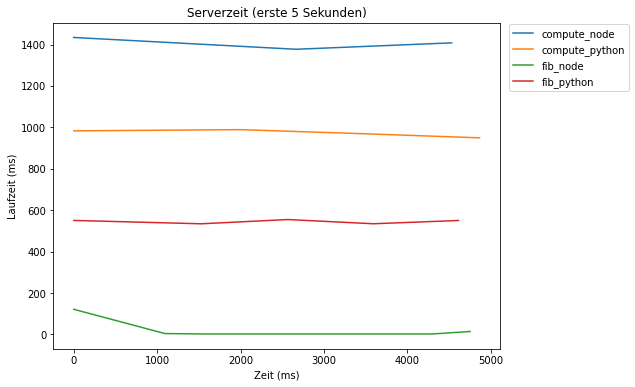
\includegraphics[scale=0.7]{aw_c_server_start}
	\captionsource{Serverseitige Laufzeiten der Lambda Funktionen (Ausschnitt)}
	{Eigene Darstellung (Matplotlib)}
	\label{aw_c_server_start}
\end{figure}
\FloatBarrier

\FloatBarrier
\begin{figure}[h!]
	\centering
	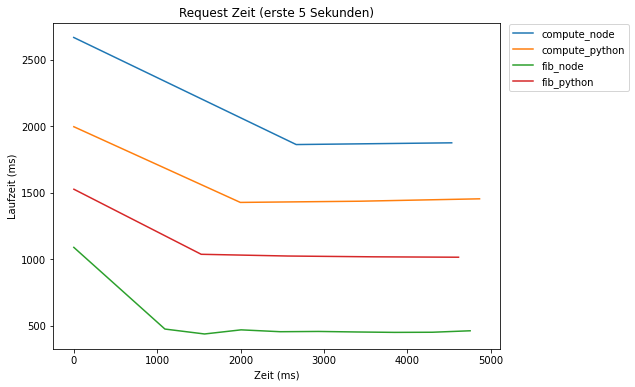
\includegraphics[scale=0.7]{aw_c_client_start}
	\captionsource{Laufzeiten des gesamten Funktionsaufrufs (Ausschnitt)}
	{Eigene Darstellung (Matplotlib)}
	\label{aw_c_client_start}
\end{figure}
\FloatBarrier

In dem in Grafik \ref{aw_c_client_start} gezeigten Ausschnitt wird die Start erhöhte Latenz der ersten Abfrage besonders deutlich. Zudem fällt auf dass die NodeJS Fibonacci Implementierung die größte Verzögerung aufweist. Dies lässt sich mit einem Blick in Grafik \ref{aw_c_server_start} erklären, da die Funktion bei ihrer ersten Ausführung bereits eine erhöhte Laufzeit aufweist, summiert sich diese mit der Kaltstartverzögerung.

\subsection{AWS Cloudwatch}

Neben den von der Testanwendung gesammelten Daten, können ebenfalls die von AWS gesammelten Log Daten der Lambda Funktionen analysiert werden. Diese können mithilfe des AWS CloudWatch Service eingesehen und als CSV exportiert werden. 

\FloatBarrier
\begin{figure}[h!]
	\centering
	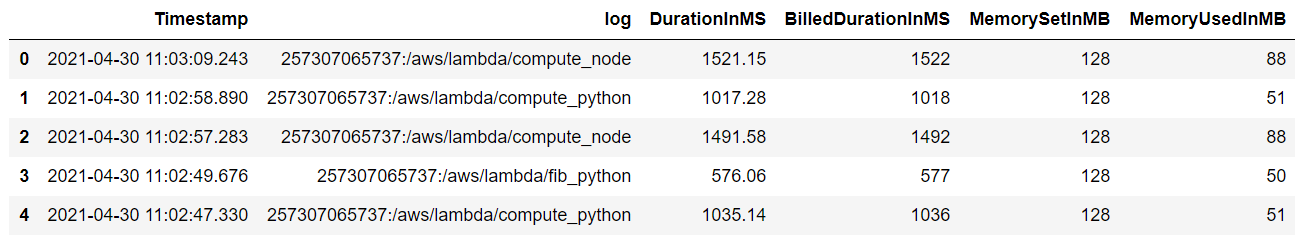
\includegraphics[width=15cm, height=3cm]{CloudWatchDataExample}
	\captionsource{Ausschnitt aus den von AWS CloudWatch gesammelten Daten}
	{Eigene Darstellung (Pandas), Daten von AWS CloudWatch bereitgestellt}
	\label{CloudWatchDFHead}
\end{figure}
\FloatBarrier

Stellt man diese Daten ebenfalls graphisch dar, so erhält man folgende Übersicht:

\FloatBarrier
\begin{figure}[h!]
	\centering
	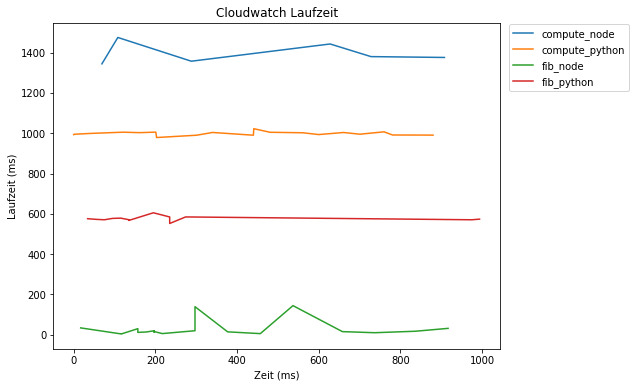
\includegraphics[scale=0.7]{aw_c_cloudwatch}
	\captionsource{AWS CloudWatch Laufzeiten}
	{Eigene Darstellung (Matplotlib), Daten von AWS CloudWatch bereitgestellt}
	\label{aw_c_cloudwatch}
\end{figure}
\FloatBarrier

Die von AWS bereitgestellten Daten bestätigen die von den Funktionen selbst gemessenen Laufzeiten. Neben den Laufzeiten misst Cloudwatch ebenfalls den Speicherverbrauch der Funktionen.

\FloatBarrier
\begin{figure}[h!]
	\centering
	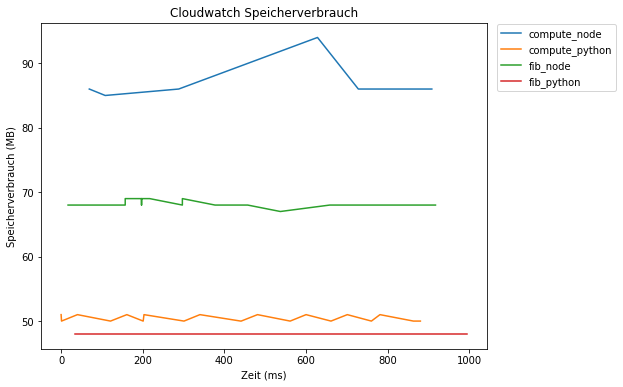
\includegraphics[scale=0.7]{aw_c_cloudwatch_ram}
	\captionsource{AWS CloudWatch Speicherverbrauch}
	{Eigene Darstellung (Matplotlib), Daten von AWS CloudWatch bereitgestellt}
	\label{aw_c_cloudwatch_ram}
\end{figure}
\FloatBarrier

Abbildung \ref{aw_c_cloudwatch_ram} zeigt den Speicherverbrauch der Funktionen. Hier fällt der deutlich höhere Speicherverbrauch der NodeJS Funktionen auf, was auf die Unterschiede zwischen dem NodeJS Framework und Python zurückzuführen ist.  

\newpage
\subsection{Coldstart Abweichungen}

Berechnet man die Abweichung in der Laufzeit der ersten Abfrage verglichen mit dem Durchschnitt aller anderen Abfragen so erhält man folgende Werte:
\\
\begin{table}[h!]
	\centering
	\begin{tabular}{||c c||} 
		\hline
		Funktion & Absolute Abweichung \\ [0.5ex] 
		\hline\hline
		compute\_node & 798.0ms \\
		compute\_python & 557.0ms \\
		fib\_node & 632.0ms \\
		fib\_python & 503.0ms \\ [1ex] 
		\hline
	\end{tabular}

	\vspace{1cm}

	\begin{tabular}{||c c||} 
		\hline
		Funktion & Relative Abweichung \\ [0.5ex] 
		\hline\hline
		compute\_node & 70\% \\
		compute\_python & 72\% \\
		fib\_node & 42\% \\
		fib\_python & 67\% \\ [1ex] 
		\hline
	\end{tabular}
	\caption{Auswirkungen des Coldstart}
	\label{table:2}
\end{table}

Der Tabelle lässt sich entnehmen, das die durchschnittliche Kaltstartverzögerung der untersuchten Funktionen zwischen 42\% und 72\% der normalen Laufzeit liegt.


\newpage
\section{Schlussfolgerungen}

Aus den durchgeführten Versuchen kann man schließen, dass es bei AWS Lambda-Funktionen ein Coldstart verhalten gibt. Allerdings scheint Lambda so weitgehend Optimiert, dass man nur bei der allerersten Abfrage nach einer längeren Wartezeit eine deutliche Verzögerung feststellen kann. Daher betrifft die Kaltstart Problematik nur selten genutzte Funktionen die genügend Lehrlauf besitzen damit sie auf null Instanzen skaliert werden.
\\
Bei den verwendeten Testfunktionen mit durchschnittlichen (serverseitigen) Laufzeiten zwischen wenigen Millisekunden und ca 1.4 Sekunden trat eine relative Verzögerung zwischen 40\% und 70\% auf. Diese ist allerdings nur Clientseitig messbar, da die tatsächliche Laufzeit der Funktion (nach Instanziierung) fast unverändert ist.
\\
Weitere Untersuchungen für komplexeren Funktionen, die weitere AWS Services einbinden (z.B Datenbankabfragen) bieten sich für zukünftige Versuche an, da die Auswirkungen dieser Services auf das Kaltstartverhalten nicht untersucht wurden.
 


\newpage

\nocite{*}
\thispagestyle{headings}

\bibliographystyle{IEEEtr}
\bibliography{bibo} 

\end{document}